\documentclass[8pt,a4paper,compress,handout]{beamer}

\usepackage{/home/siyer/lib/slides}

\title{Defining Functions}
\date{}

\begin{document}
\begin{frame}
\hfill
\begin{minipage}{150pt}
\begin{flushright}
\tiny \emph{It's OK to figure out murder mysteries, but you shouldn't need to figure out code. You should be able to read it.}

\smallskip

- Steve McConnell
\end{flushright}
\end{minipage}
\vfill
\titlepage
\end{frame}

\begin{frame}
\frametitle{Outline}
\tableofcontents
\end{frame}

\section{Using and Defining Functions}
\begin{frame}[fragile]
Functions allow us to:
\begin{itemize}
\item transfer control back and forth between different pieces of code; 
\item clearly separate tasks within a program; and
\item reuse code.
\end{itemize}

\bigskip

Function definition in Python:
\begin{lstlisting}[language=Python]
def <name>(<parameter name>, <parameter name>, ...):
    <statement>
    <statement>
    ...
\end{lstlisting}

\begin{itemize}
\item The first line, known as the \emph{signature}, consists of the \lstinline{def} keyword, the function name, a sequence of zero or more parameter variables separated by commas and enclosed in parentheses, and a colon.

\item The indented statements following the signature constitute the \emph{function body}.

\item The function body can contain a \emph{return statement}, which transfers control to the point where the function was called and returns the result of the computation (aka \emph{the return value}).
\end{itemize}
\end{frame}

\begin{frame}[fragile]
For example, the following function tests if the argument $N$ is prime:

\begin{lstlisting}[language=Python]
def is_prime(N):
    if N < 2: 
        return False
    i = 2
    while i <= N / i:
        if N % i == 0:
            return False
        i += 1
    return True
\end{lstlisting}

\bigskip

A \emph{function call} is its name followed by expressions that specify argument values in parentheses, separated by commas. For example, \lstinline{is_prime(31)}.

\bigskip

When the function call is part of an expression, as in \lstinline{x = math.sqrt(3)}, the function computes a value that is used in place of the call in the expression. 

\bigskip

Otherwise, the function call is a statement that generally causes side effects, as in \lstinline{stdio.writeln('Hello, World')}.

\bigskip

When a module is executed directly by the \lstinline{python} command (and not via an \lstinline{import} statement), the module's \lstinline{__name__} is set equal to \lstinline{'__main__'}.
\end{frame}

\begin{frame}[fragile]
\begin{framed}
\tiny harmonicf.py:  Write to standard output the harmonic numbers specified as command-line arguments.
\end{framed}

\begin{lstlisting}[language=Python]
import stdio
import sys

def harmonic(n):
    total = 0.0
    for i in range(1, n + 1):
        total += 1.0 / float(i)
    return total

def main():
    for j in range(1, len(sys.argv)):
        arg = int(sys.argv[j])
        value = harmonic(arg)
        stdio.writeln(value)

if __name__ == '__main__':
    main()
\end{lstlisting}

\begin{lstlisting}[language={}]
$ python harmonicf.py 1 2 4
1.0
1.5
2.08333333333
\end{lstlisting}
\end{frame}

\begin{frame}[fragile]
A Python function can have more than one parameter variable, so it can be called with more than one argument. 
\begin{lstlisting}[language=Python]
def hypot(a, b):
    return math.sqrt(a * a + b * b)
\end{lstlisting}

\bigskip

We can define as many functions as we want in a \lstinline{.py} file. 
\begin{lstlisting}[language=Python]
def square(x):
    return x * x

def hypot(a, b):
    return math.sqrt(square(a) + square(b))
\end{lstlisting}

\bigskip

We can put \lstinline{return} statements in a function wherever we need them, as in the \lstinline{is_prime()} function.

\bigskip

A function provides only one return value to the caller. More precisely, it returns a reference to one object.

\bigskip

The scope of a function's local and parameter variables is limited to that function.

\bigskip

The scope of a variable defined in global code --- known as a \emph{global variable} --- is limited to the \lstinline{.py} file containing that variable. 
\end{frame}

\begin{frame}[fragile]
A function may designate an argument to be \emph{optional} by specifying a \emph{default value} for that argument. 

\bigskip

For example, the following function computes the \emph{$n$th generalized harmonic number of order $r$}, $H_{n,r}=1+1/2^r+1/3^r+\cdots+1/n^r$:

\begin{lstlisting}[language=Python]
def harmonic(n, r = 1):
    total = 0.0
    for i in range(1, n + 1):
        total += 1.0 / (i ** r)
    return total
\end{lstlisting}
With this definition, \lstinline{harmonic(2, 2)} returns \lstinline{1.25}, while both \lstinline{harmonic(2, 1)} and \lstinline{harmonic(2)} return \lstinline{1.5}.

\bigskip

\emph{Named arguments} allow us to specify arguments to a function in any order. For example, the call \lstinline{harmonic(r = 2, n = 3)} is the same as the call \lstinline{harmonic(3, 2)}.

\bigskip

Python supports \emph{functional polymorphism}, which allows us to define a single function for use with objects of different types. For example, \lstinline{square()} when called with an integer argument, returns an integer, but when called with a float argument, returns a float.
\end{frame}

\section{Implementing Mathematical Functions}

\begin{frame}[fragile]
\begin{minipage}{200pt}
The \emph{standard normal (Gaussian) probability density function (pdf)} is characterized by the familiar bell-shaped curve defined by the formula $\phi(x)=e^{-x^2/2}/\sqrt{2\pi}$.

\bigskip

The \emph{normal (Gaussian) pdf} $\phi(x, \mu, \sigma)$ is the same as $\phi((x-\mu)/\sigma)/\sigma$. 

\bigskip

The \emph{standard normal (Gaussian) cumulative distribution function (cdf)} $\Phi(z)$ is defined to be the area under the curve defined by $\phi(x)$ above the $x$-axis and to the left of the vertical line $x=z$. 

\bigskip

No formula is known for $\Phi(z)$, but it can be approximated as follows: $$\Phi(z)=\frac{1}{2}+\phi(z)\big(z+\frac{z^3}{3}+\frac{z^5}{3\cdot 5}+\frac{z^7}{3\cdot 5\cdot 7}+\cdots\big ).$$
\end{minipage}\hfill%
\begin{minipage}{100pt}
\begin{center}
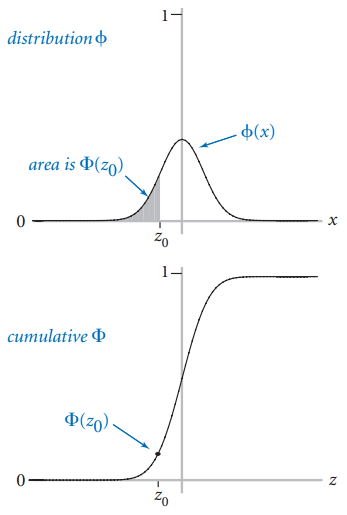
\includegraphics[scale=0.25]{figures/gaussian.png}

\smallskip

\tiny

Gaussian probability functions
\end{center}
\end{minipage}
\end{frame}

\begin{frame}[fragile]
\begin{framed}
\tiny gauss.py: Accept floats $z$, $mu$, and $sigma$ as command-line arguments. Use them to test the normal (Gaussian) probability density (pdf) cumulative distribution (cdf) functions. Write the results to standard output.
\end{framed}

\begin{lstlisting}[language=Python]
import math
import stdio
import sys

def phi(x):
    return math.exp(- x * x / 2.0) / math.sqrt(2.0 * math.pi)

def pdf(x, mu = 0.0, sigma = 1.0):
    return phi((x - mu) / sigma) / sigma

def Phi(z):
    if z < -8.0:
        return 0.0
    if z > 8.0:
        return 1.0
    total = 0.0
    term = z
    i = 3
    while total != total + term:
        total += term
        term *= z * z / float(i)
        i += 2
    return 0.5 + phi(z) * total

def cdf(z, mu = 0.0, sigma = 1.0):
    return Phi((z - mu) / sigma)
\end{lstlisting}
\end{frame}

\begin{frame}[fragile]
\begin{lstlisting}[language=Python]
def main():
    z = float(sys.argv[1])
    mu = float(sys.argv[2])
    sigma = float(sys.argv[3])
    stdio.writeln(cdf(z, mu, sigma))

if __name__ == '__main__':
    main()
\end{lstlisting}

\begin{lstlisting}[language={}]
$ python gauss.py 820 1019 209
0.170509668691
$ python gauss.py 1500 1019 209
0.989316483738
$ python gauss.py 1500 1025 231
0.980122090737
\end{lstlisting}
\end{frame}

\section{Using Functions to Organize Code}

\begin{frame}[fragile]
\begin{framed}
\tiny coupon.py: Accept integer $n$ as a command-line argument. Write to standard output the number of coupons collected before obtaining one of each of $n$ types.
\end{framed}

\begin{lstlisting}[language=Python]
import random
import stdarray
import stdio
import sys

def getCoupon(n):
    return random.randrange(0, n)

def collect(n):
    found = stdarray.create1D(n, False)
    couponCount = 0
    distinctCouponCount = 0
    while distinctCouponCount < n:
        coupon = getCoupon(n)
        couponCount += 1
        if not found[coupon]:
            distinctCouponCount += 1
            found[coupon] = True
    return couponCount

def main():
    n = int(sys.argv[1])
    couponCount = collect(n)
    stdio.writeln(couponCount)

if __name__ == '__main__':
    main()
\end{lstlisting}
\end{frame}

\begin{frame}[fragile]
\begin{lstlisting}[language={}]
$ python coupon.py 1000
5193
$ python coupon.py 1000
6865
$ python coupon.py 1000000
15490879
\end{lstlisting}
\end{frame}

\section{Passing Arguments and Returning Values}
\begin{frame}[fragile]
We can use parameter variables anywhere in the body of the function in the same way as we use local variables. 

\bigskip

Python initializes the parameter variable with the corresponding argument provided by the calling code --- an approach known as \emph{call by object reference} (aka \emph{call by value}).

\bigskip

As a consequence, if a parameter variable refers to a mutable object and we change that object's value within a function, then this also changes the object's value in the calling code.

\bigskip

When a function takes a list as an argument, it implements a function that operates on an arbitrary number of objects. 
\begin{lstlisting}[language=Python]
def mean(a):
    total = 0.0
    for v in a:
        total += v
    return total / len(a)
\end{lstlisting}
\end{frame}

\begin{frame}[fragile]
Since lists are \emph{mutable}, it is often the case that the purpose of a function that takes a list as argument is to produce a side effect.
\begin{lstlisting}[language=Python]
def exchange(a, i, j):
    temp = a[i]
    a[i] = a[j]
    a[j] = temp
\end{lstlisting}

\bigskip

There are situations where it is useful for a function to return a list.
\begin{lstlisting}[language=Python]
def randomarray(n):
    a = stdarray.create1D(n)
    for i in range(n):
        a[i] = random.random()
    return a
\end{lstlisting}
\end{frame}

\begin{frame}[fragile]
\begin{framed}
\tiny playthattunedeluxe.py: Read sound samples from standard input, add harmonics, and play the resulting sound to standard audio.
\end{framed}

\begin{lstlisting}[language=Python]
import math
import stdarray
import stdaudio
import stdio

def superpose(a, b, aWeight, bWeight):
    c = stdarray.create1D(len(a), 0.0)
    for i in range(len(a)):
        c[i] = a[i] * aWeight + b[i] * bWeight
    return c

def tone(hz, t):
    SPS = 44100
    n = int(SPS * t)
    a = stdarray.create1D(n + 1, 0.0)
    for i in range(n + 1):
        a[i] = math.sin(2.0 * math.pi * i * hz / SPS)
    return a

def note(pitch, t):
    CONCERT_A_HZ = 440.0
    NOTES_ON_SCALE = 12.0
    hz = CONCERT_A_HZ * (2.0 ** (pitch / NOTES_ON_SCALE))
    a = tone(hz, t)
    hi = tone(2 * hz, t)
    lo = tone(hz / 2, t)
    h = superpose(hi, lo, .5, .5)
    return superpose(a, h, .5, .5)
\end{lstlisting}
\end{frame}

\begin{frame}[fragile]
\begin{lstlisting}[language=Python]
def main():
    while not stdio.isEmpty():
        pitch = stdio.readInt()
        duration = stdio.readFloat()
        a = note(pitch, duration)
        stdaudio.playSamples(a)
    stdaudio.wait()

if __name__ == '__main__':
    main()
\end{lstlisting}

\begin{minipage}{170pt}
\begin{lstlisting}[language={}]
$ head -5 elise.txt
7 .125 
6 .125 
7 .125 
6 .125 
7 .125 
$ python playthattunedeluxe.py < elise.txt
\end{lstlisting}
\end{minipage}%
\begin{minipage}{130pt}
\hfill 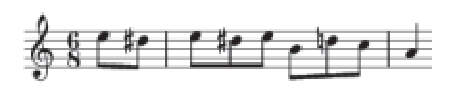
\includegraphics[scale=0.5]{figures/furelise.pdf}
\end{minipage}
\end{frame}

\section{Filter, Lambda, Map, and Reduce Functions}
\begin{frame}[fragile]
In Python, functions are \emph{first-class citizens}, meaning they are actually data just like numbers, lists, and strings.

\bigskip

As a result, we can write functions that take \emph{other functions} as arguments and return \emph{other functions} as results.

\bigskip

The built-in function \lstinline{filter(f, seq)} returns those items of the sequence \lstinline{seq} for which \lstinline{f(item)} is \lstinline{True}. 
\begin{lstlisting}[language={}]
>>> primes = filter(is_prime, range(11))
>>> primes
[2, 3, 5, 7]
\end{lstlisting}

\bigskip

A \emph{lambda function} is a ``disposable'' function that we can define just when we need it and then immediately throw it away after we are done using it. 
\begin{lstlisting}[language={}]
>>> odds = filter(lambda x : x % 2 != 0, range(11))
>>> odds
[1, 3, 5, 7, 9]
\end{lstlisting}
\end{frame}

\begin{frame}[fragile]
The built-in function \lstinline{map(f, seq)} returns a list of the results of applying the function \lstinline{f} to the items of the sequence \lstinline{seq}.
\begin{lstlisting}[language={}]
squares = map(lambda x : x ** 2, range(11))
>>> squares
[0, 1, 4, 9, 16, 25, 36, 49, 64, 81, 100]
\end{lstlisting}

\bigskip

The built-in function \lstinline{reduce(f, seq)} applies a function \lstinline{f} of two arguments cumulatively to the items of a sequence \lstinline{seq}, from left to right, so as to reduce the sequence to a single value.
\begin{lstlisting}[language={}]
>>> total = reduce(lambda x, y: x + y, range(11))
>>> total
55
\end{lstlisting}
\end{frame}

\begin{frame}[fragile]
\begin{framed}
\tiny cryptography.py: A module that implements RSA cryptography.
\begin{itemize}

\item A message $x$ is encrypted using the function $f(x) = x^e \bmod n$, where $n=pq$ for two different large primes $p$ and $q$ chosen at random, and $e$ is a random prime number less than $m=(p-1)(q-1)$ such that $e$ does not divide $m$. 

\item The maximum number that can be encrypted is $n-1$.

\item Together, the values $e$ and $n$ are called the \emph{public key}.

\item A message $y$ is decrypted using the function $g(y) = y^d \bmod n$, where $d \leq m-1$ is the multiplicative inverse of $e \bmod m$, ie, $ed \bmod m = 1$.

\item The value $d$ is called the \emph{private key}.
\end{itemize}
\end{framed}
\begin{lstlisting}[language=Python]
import random
import stdio

def is_prime(N):
    if N < 2: 
        return False
    i = 2
    while i <= N / i:
        if N % i == 0:
            return False
        i += 1
    return True

def primes(N):
    return filter(is_prime, range(N))
\end{lstlisting}
\end{frame}

\begin{frame}[fragile]
\begin{lstlisting}[language=Python]
def inverse(e, m):
    return filter(lambda d: e * d % m == 1, range(1, m))[0]

def make_encoder_decoder(N):
    p, q = random.sample(primes(N), 2)
    n = p * q
    m = (p - 1) * (q - 1)
    stdio.writef('Maximum number that can be encrypted is %d\n', n - 1)
    e = random.choice(primes(m))
    while m % e == 0:
        e = random.choice(primes(m))
    d = inverse(e, m)
    encoder = lambda x: (x ** e) % n
    decoder = lambda y: (y ** d) % n
    return [encoder, decoder]
\end{lstlisting}

\begin{lstlisting}[language={}]
>>> import cryptography
>>> encoder, decoder = cryptography.make_encoder_decoder(100)
Maximum number that can be encrypted is 2536
>>> encoder(42)
2235L
>>> decoder(2235)
42L
>>> decoder(encoder(1729))
1729L
\end{lstlisting}
\end{frame}
\end{document}
